\documentclass{standalone}
\usepackage{fontspec}
\setsansfont{DejaVuSans.ttf}[Path=./,Kerning=Off,Ligatures={TeXOff,NoCommon}]
\usepackage{tikz}
\begin{document}
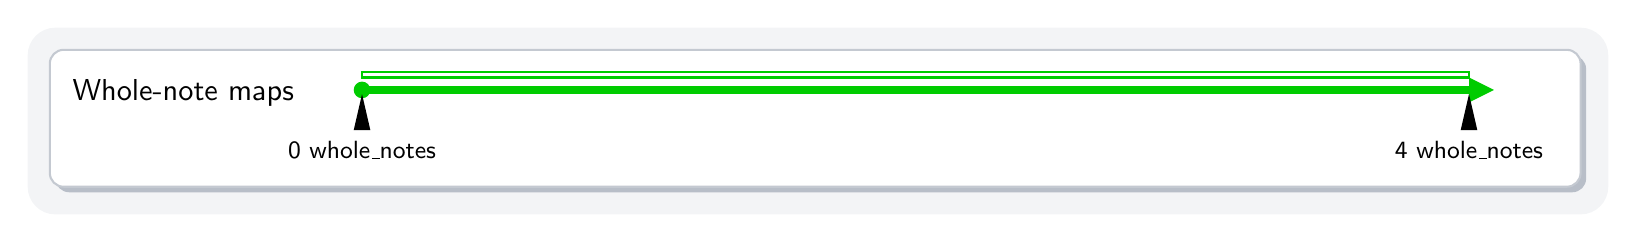
\begin{tikzpicture}[x=1pt,y=1pt,miter limit=4,font=\sffamily]
\definecolor{ts000000}{HTML}{000000}
\definecolor{ts00CC00}{HTML}{00CC00}
\definecolor{tsB8BEC8}{HTML}{B8BEC8}
\definecolor{tsC4C9D1}{HTML}{C4C9D1}
\definecolor{tsF3F4F6}{HTML}{F3F4F6}
\definecolor{tsFFFFFF}{HTML}{FFFFFF}
\begin{scope}[shift={(16,16)}]
\path[rounded corners=10pt,fill=tsF3F4F6] (0,0) rectangle (571.1499,67.4766);
\path[rounded corners=5pt,fill=tsB8BEC8] (10,8) rectangle (563.1499,57.4766);
\path[rounded corners=5pt,fill=tsFFFFFF,draw=tsC4C9D1,line width=0.75pt] (8,10) rectangle (561.1499,59.4766);
\path[draw=ts00CC00,line width=1pt] (120.8193,51.4766) -- (520.8193,51.4766) -- (520.8193,49.4766) -- (120.8193,49.4766) -- cycle;
\path[draw=ts00CC00,line width=3pt] (120.8193,44.9766) -- (520.8193,44.9766);
\path[fill=ts00CC00] (120.8193,44.9766) circle[radius=3];
\path[fill=ts00CC00] (529.8193,44.9766) -- (520.8193,49.4766) -- (520.8193,40.4766) -- cycle;
\path[fill=ts000000] (120.8193,43.4766) -- (117.8193,30.4766) -- (123.8193,30.4766) -- cycle;
\path[fill=ts000000] (520.8193,43.4766) -- (517.8193,30.4766) -- (523.8193,30.4766) -- cycle;
\node[anchor=base west,inner sep=0,font=\sffamily\fontsize{11}{12.8047}\selectfont,text=ts000000] at (16,41.1685) {Whole-note maps};
\node[anchor=base,inner sep=0,font=\sffamily\fontsize{9}{10.4766}\selectfont,text=ts000000] at (120.8193,20.1226) {0 whole\_notes};
\node[anchor=base,inner sep=0,font=\sffamily\fontsize{9}{10.4766}\selectfont,text=ts000000] at (520.8193,20.1226) {4 whole\_notes};
\end{scope}
\end{tikzpicture}
\end{document}
